% Generazione delle variabili che andranno a sostituire quelle del template `HomePage.tex`
\newcommand{\documento}{\MS}
\newcommand{\nomedocumentofisico}{\MSv.pdf}
\newcommand{\redazione}{\TG \\ & \CV}
\newcommand{\verifica}{\LC \\ & \NC}
\newcommand{\approvazione}{\SG}
\newcommand{\versione}{1.0.0}
\newcommand{\uso}{Esterno}
\newcommand{\destinateTo}{\TV, \\ & \RC, \\ & \II}
\newcommand{\datacreazione}{02 aprile 2019}
\newcommand{\datamodifica}{02 aprile 2019}
\newcommand{\stato}{Approvato}

\def\TABELLE{true}	% abilita - disabilita l'indice delle tabelle
\def\FIGURE{true} 	% abilita - disabilita l'indice delle figure


\documentclass[a4paper,11pt]{article}

\usepackage{ifthen}
\usepackage[english,italian]{babel}
\usepackage[utf8]{inputenc}
\usepackage[T1]{fontenc}
\usepackage{float}
\usepackage{chapterbib}
\usepackage{graphicx}
\usepackage[a4paper,top=2.5cm,bottom=2.5cm,left=2.5cm,right=2.5cm]{geometry}

\PassOptionsToPackage{hyphens}{url}\usepackage[hyperfootnotes=false]{hyperref}
\hypersetup{%
	colorlinks=true,
	citecolor=black,
	linkcolor=black,
	urlcolor=blue
}

\usepackage{enumitem}
\usepackage{eurosym}
\usepackage{booktabs}
\usepackage{fancyhdr}
\usepackage{totpages}
\usepackage{tabularx, array}
\usepackage{dcolumn}
\usepackage{epstopdf}
\usepackage{booktabs}
\usepackage{fancyhdr}
\usepackage{longtable}
\usepackage{calc}
\usepackage{datatool}
\usepackage[bottom]{footmisc}
\usepackage{listings}
\usepackage{textcomp}
\usepackage{titlesec}
\usepackage{rotating}
\usepackage{multirow}
\usepackage{placeins}
\usepackage{color}
\usepackage{makecell}
\usepackage{lscape}
 
\usepackage[table,usenames,dvipsnames]{xcolor}
% Definizione di nuovi colori da poter usare per le tabelle
\definecolor{lightgray}{gray}{0.92}
\definecolor{lightblue}{rgb}{0.93,0.95,1.0}
\definecolor{headgray}{gray}{0.88}

% Ridefinizione dell'env tabularx. Il vecchio è utilizzabile con l'env oldtabularx
\let\oldtabularx\tabularx
\let\endoldtabularx\endtabularx
\renewenvironment{tabularx}{\rowcolors{2}{white}{lightgray}\oldtabularx}{\endoldtabularx}

% Per tabularx con padding, parametro tra [], eg [1.3]
\newenvironment{paddedtablex}[1][1]{%
	\renewcommand*{\arraystretch}{#1}%
	\renewcommand\theadfont{\bfseries}%
	\tabularx%
}{%
	\endtabularx
}

% Ridefinizione dell'env tabular. Il vecchio è utilizzabile con l'env oldtabular
\let\oldtabular\tabular
\let\endoldtabular\endtabular
\renewenvironment{tabular}{\rowcolors{2}{lightgray}{white}\oldtabular}{\endoldtabular}

% Per tabular con padding, parametro tra [], eg [1.3]
\newenvironment{paddedtable}[1][1]{%
	\renewcommand*{\arraystretch}{#1}%
	\renewcommand\theadfont{\bfseries}%
	\tabular%
}{%
	\endtabular
}

% ***TABELLA ANALISI RISCHI PDP***

\newenvironment{risktable}[1][1]{%
	\centering%
	\renewcommand*{\arraystretch}{1.4}%
	\renewcommand\theadfont{\bfseries}%
	\oldtabularx%
}{%
	\endoldtabularx
}

% ***TABELLA SUDDIVISIONE DEL LAVORO PDP***

\newenvironment{detailtable}[1][1]{%
	\centering%
	\renewcommand*{\arraystretch}{1.4}%
	\renewcommand\theadfont{\bfseries}%
	\oldtabularx%
}{%
	\endoldtabularx
}

% ***TABELLA ORGANIGRAMMA***

\newenvironment{orgtable}[1][1]{%
	\centering%
	\renewcommand*{\arraystretch}{1.4}%
	\renewcommand\theadfont{\bfseries}%
	\oldtabularx%
}{%
	\endoldtabularx
}


% DA SPOSTARE SU COMANDI
% ***DOUBLE LINE***

\def\mydoublerule#1#2#3{%%
	\hrule width#1 height#2 \vskip#2
	\hrule width#1 height#3 
}

% ***NUOVO TIPO DI CELLA CENTRATA***

\newcolumntype{Y}{>{\centering\arraybackslash}X}

% ***STILE PAGINA***
\pagestyle{fancy}

% ***INTESTAZIONE***
\rhead{\Large{\progetto} \\ \footnotesize{\documento}}
\lhead{
\includegraphics[keepaspectratio = true, width = 25px]{../template/icons/a6(1).png}}

% ***PIÈ DI PAGINA***
\lfoot{\textit{\gruppo} \\
\footnotesize{\email}}

\rfoot{\thepage} % per le prime pagine: mostra solo il numero romano
\cfoot{}
\renewcommand{\footrulewidth}{0.4pt}   % Linea sopra il piè di pagina
\renewcommand{\headrulewidth}{0.4pt}  % Linea sotto l'intestazione

% ***INSERIMENTO DI NUOVE SOTTOSEZIONI
\setcounter{secnumdepth}{7} %mostra nel documento fino al livello 8 (1.2.3.4.5.6.7.8)
\setcounter{tocdepth}{7}    % mostra nell'indice fino al livello 8 (1.2.3.4.5.6.7.8)


\makeatletter
\newcounter{subsubparagraph}[subparagraph]
\renewcommand\thesubsubparagraph{%
	\thesubparagraph.\@arabic\c@subsubparagraph}
\newcommand\subsubparagraph{%
	\@startsection{subsubparagraph}    % counter
	{6}                              % level
	{\parindent}                     % indent
	{3.25ex \@plus 1ex \@minus .2ex} % beforeskip
	{0.75em}                           % afterskip
	{\normalfont\normalsize\bfseries}}
\newcommand\l@subsubparagraph{\@dottedtocline{6}{10em}{5.5em}} %gestione dell'indice
\newcommand{\subsubparagraphmark}[1]{}
\makeatother

\makeatletter
\newcounter{subsubsubparagraph}[subsubparagraph]
\renewcommand\thesubsubsubparagraph{%
	\thesubsubparagraph.\@arabic\c@subsubsubparagraph}
\newcommand\subsubsubparagraph{%
	\@startsection{subsubsubparagraph}    % counter
	{7}                              % level
	{\parindent}                     % indent
	{3.25ex \@plus 1ex \@minus .2ex} % beforeskip
	{0.75em}                           % afterskip
	{\normalfont\normalsize\bfseries}}
\newcommand\l@subsubsubparagraph{\@dottedtocline{7}{10em}{6.5em}} %gestione dell'indice
\newcommand{\subsubsubparagraphmark}[1]{}
\makeatother

 % Layout del documento
% Generali
\newcommand{\progetto}{Butterfly}
\newcommand{\gruppo}{AlphaSix}
\newcommand{\email}{alpha.six.unipd@gmail.com}

% Documenti
\newcommand{\AdR}{Analisi dei Requisiti}
\newcommand{\NdP}{Norme di Progetto}
\newcommand{\PdP}{Piano di Progetto}
\newcommand{\SdF}{Studio di Fattibilità}
\newcommand{\PdQ}{Piano di Qualifica}
\newcommand{\VI}{Verbale Interno}
\newcommand{\VE}{Verbale Esterno}
\newcommand{\ST}{Specifica Tecnica}
\newcommand{\DDP}{Definizione di Prodotto}
\newcommand{\MU}{Manuale Utente}
\newcommand{\Gl}{Glossario}
\newcommand{\LdP}{Lettera di Presentazione}
\newcommand{\AdRv}{AnalisiDeiRequisiti v2.0.0}
\newcommand{\NdPv}{NormeDiProgetto v2.0.0}
\newcommand{\PdPv}{PianoDiProgetto v2.0.0}
\newcommand{\PdQv}{PianoDiQualifica v2.0.0}
\newcommand{\SdFv}{StudioDiFattibilità v1.0.0}
\newcommand{\DdPv}{DefinizioneDiprodotto v1.0.0}
\newcommand{\Glv}{Glossario v2.0.0}

% Componenti del gruppo
\newcommand{\LC}{Laura Cameran}
\newcommand{\TG}{Timoty Granziero}
\newcommand{\CV}{Ciprian Voinea}
\newcommand{\SG}{Samuele Gardin}
\newcommand{\NC}{Nicola Carlesso}
\newcommand{\MM}{Matteo Marchiori}

% Ruoli
\newcommand{\RdP}{Responsabile di Progetto}
\newcommand{\Res}{Responsabile}
\newcommand{\Red}{Redattore}
\newcommand{\Amm}{Amministratore}
\newcommand{\Ver}{Verificatore}
\newcommand{\Prog}{Progettista}
\newcommand{\Progr}{Programmatore}
\newcommand{\Ana}{Analista}
\newcommand{\RdPs}{Responsabili di Progetto}
\newcommand{\Ress}{Responsabile}
\newcommand{\Amms}{Amministratori}
\newcommand{\Vers}{Verificatori}
\newcommand{\Progs}{Progettisti}
\newcommand{\Progrs}{Programmatori}
\newcommand{\Anas}{Analisti}

% Professori e proponente
\newcommand{\TV}{Prof. Tullio Vardanega}
\newcommand{\RC}{Prof. Riccardo Cardin}
\newcommand{\LuC}{Luca Cappelletti}
\newcommand{\DZ}{Davide Zanetti}
\newcommand{\II}{Imola Informatica}
\newcommand{\proponente}{Imola Informatica}

% Comando per una nuova riga nella tabella del diario delle modifiche
\newcommand{\specialcell}[2][c]{%
	\begin{tabular}[#1]{@{}c@{}}#2\end{tabular}}

\renewcommand*\sectionmark[1]{\markboth{#1}{}}
\renewcommand*\subsectionmark[1]{\markright{#1}}

% Pediodi di lavoro 
\newcommand{\AR}{Analisi dei Requisiti}
\newcommand{\AD}{Analisi dei Requisiti in Dettaglio}
\newcommand{\PA}{Progettazione Architetturale}
\newcommand{\PD}{Progettazione di Dettaglio}
\newcommand{\CO}{Codifica}
\newcommand{\VV}{Validazione}

% Revisioni
\newcommand{\RR}{Revisione dei Requisiti}
\newcommand{\RP}{Revisione di Progettazione}
\newcommand{\RQ}{Revisione di Qualifica}
\newcommand{\RA}{Revisione di Accettazione}

\newcommand{\myincludegraphics}[2][]{%
	\setbox0=\hbox{\phantom{X}}%
	\vtop{
		\hbox{\phantom{X}}
		\vskip-\ht0
		\hbox{\includegraphics[#1]{#2}}}}

% Ridefinizione linea per le note a piè di pagina
\renewcommand{\footnoterule}{%
  \kern -3pt
  \hrule width \textwidth height 0.4pt
  \kern 2pt
}

\colorlet{punct}{red!60!black}
\definecolor{background}{HTML}{EEEEEE}
\definecolor{delim}{RGB}{20,105,176}
\colorlet{numb}{magenta!60!black}
\lstdefinelanguage{json}{
 	basicstyle=\small\ttfamily,
 	numbers=left,
 	numberstyle=\scriptsize,
 	stepnumber=1,
 	numbersep=8pt,
 	showstringspaces=false,
 	breaklines=true,
 	frame=lines,
 	backgroundcolor=\color{background},
 	literate=
 	*{0}{{{\color{numb}0}}}{1}
 	{1}{{{\color{numb}1}}}{1}
 	{2}{{{\color{numb}2}}}{1}
 	{3}{{{\color{numb}3}}}{1}
 	{4}{{{\color{numb}4}}}{1}
 	{5}{{{\color{numb}5}}}{1}
 	{6}{{{\color{numb}6}}}{1}
 	{7}{{{\color{numb}7}}}{1}
 	{8}{{{\color{numb}8}}}{1}
 	{9}{{{\color{numb}9}}}{1}
 	{:}{{{\color{punct}{:}}}}{1}
 	{,}{{{\color{punct}{,}}}}{1}
 	{\{}{{{\color{delim}{\{}}}}{1}
 	{\}}{{{\color{delim}{\}}}}}{1}
 	{[}{{{\color{delim}{[}}}}{1}
 	{]}{{{\color{delim}{]}}}}{1},
}
\lstset{language=json}
\lstset{literate=%
    {Ö}{{\"O}}1
 	{Ä}{{\"A}}1
 	{Ü}{{\"U}}1
 	{é}{{\"s}}1
 	{è}{{\"e}}1
 	{à}{{\"a}}1
	{ö}{{\"o}}1
}


\definecolor{listinggray}{gray}{0.9}
\definecolor{lbcolor}{rgb}{0.9,0.9,0.9}

\lstset{
  backgroundcolor=\color{lbcolor},
  tabsize=4,
  language=Python,
  captionpos=b,
  frame=single,
  numbers=left,
  numberstyle=\tiny,
  numbersep=5pt,
  breaklines=true,
  showstringspaces=false,
  basicstyle=\footnotesize,
  % identifierstyle=\color{magenta},
  keywordstyle=\bfseries\color[rgb]{0,0,1},
  commentstyle=\color[rgb]{0,0.6,0},
  stringstyle=\color{red}
}

% \definecolor{mygreen}{rgb}{0,0.6,0}
% \definecolor{mygray}{rgb}{0.5,0.5,0.5}
% \definecolor{mymauve}{rgb}{0.58,0,0.82}

% \lstset{ 
%   backgroundcolor=\color{white},   % choose the background color; you must add \usepackage{color} or \usepackage{xcolor}; should come as last argument
%   basicstyle=\footnotesize,        % the size of the fonts that are used for the code
%   breakatwhitespace=false,         % sets if automatic breaks should only happen at whitespace
%   breaklines=true,                 % sets automatic line breaking
%   captionpos=b,                    % sets the caption-position to bottom
%   commentstyle=\color{mygreen},    % comment style
%   deletekeywords={...},            % if you want to delete keywords from the given language
%   escapeinside={\%*}{*)},          % if you want to add LaTeX within your code
%   extendedchars=true,              % lets you use non-ASCII characters; for 8-bits encodings only, does not work with UTF-8
%   firstnumber=1000,                % start line enumeration with line 1000
%   frame=single,	                   % adds a frame around the code
%   keepspaces=true,                 % keeps spaces in text, useful for keeping indentation of code (possibly needs columns=flexible)
%   keywordstyle=\color{blue},       % keyword style
%   language=Octave,                 % the language of the code
%   morekeywords={*,...},            % if you want to add more keywords to the set
%   numbers=left,                    % where to put the line-numbers; possible values are (none, left, right)
%   numbersep=5pt,                   % how far the line-numbers are from the code
%   numberstyle=\tiny\color{mygray}, % the style that is used for the line-numbers
%   rulecolor=\color{black},         % if not set, the frame-color may be changed on line-breaks within not-black text (e.g. comments (green here))
%   showspaces=false,                % show spaces everywhere adding particular underscores; it overrides 'showstringspaces'
%   showstringspaces=false,          % underline spaces within strings only
%   showtabs=false,                  % show tabs within strings adding particular underscores
%   stepnumber=2,                    % the step between two line-numbers. If it's 1, each line will be numbered
%   stringstyle=\color{mymauve},     % string literal style
%   tabsize=2,	                   % sets default tabsize to 2 spaces
%   title=\lstname                   % show the filename of files included with \lstinputlisting; also try caption instead of title
% }

\newcommand{\impl}{\textcolor{Green}{Implementato}}
\newcommand{\implno}{\textcolor{Red}{Non Implementato}}

% G di glossario a pedice, con e senza spazio
\newcommand{\GAlt}{\ped{\tiny{G}}}
\newcommand{\G}{\ped{\tiny{G }}}

% e.g. \gloss{progetto}
\newcommand{\gloss}[1]{%
    {\small \textsc{#1}}\GAlt%
}

% D di documento a pedice, con e senza spazio
% \newcommand{\DAlt}{\ped{\tiny{D}}}
\newcommand{\D}{\ped{\tiny{D}}}

% e.g. \Doc{Norme di Progetto}
\newcommand{\Doc}[1]{\textit{#1}\D}

% Comandi per applicare \Doc con un comando unico
\newcommand{\PdQd}{\Doc{\PdQv}}
\newcommand{\PdPd}{\Doc{\PdPv}}
\newcommand{\NdPd}{\Doc{\NdPv}}
\newcommand{\AdRd}{\Doc{\AdRv}}
\newcommand{\SdFd}{\Doc{\SdFv}}
\newcommand{\Gld}{\Doc{\Gld}}

% Le sottosezioni paragraph, subparagraph ecc.. vengono visualizzate come section
\titleformat{\paragraph}{\normalfont\normalsize\bfseries}{\theparagraph}{1em}{}
\titlespacing*{\paragraph}{0pt}{3.25ex plus 1ex minus .2ex}{1.5ex plus .2ex}

\titleformat{\subparagraph}{\normalfont\normalsize\bfseries}{\thesubparagraph}{1em}{}
\titlespacing*{\subparagraph}{0pt}{3.25ex plus 1ex minus .2ex}{1.5ex plus .2ex}

\titleformat{\subsubparagraph}{\normalfont\normalsize\bfseries}{\thesubsubparagraph}{1em}{}
\titlespacing*{\subsubparagraph}{0pt}{3.25ex plus 1ex minus .2ex}{1.5ex plus .2ex}

\titleformat{\subsubsubparagraph}{\normalfont\normalsize\bfseries}{\thesubsubsubparagraph}{1em}{}
\titlespacing*{\subsubsubparagraph}{0pt}{3.25ex plus 1ex minus .2ex}{1.5ex plus .2ex}


% Indentazione paragrafi rimossa. Per metterla manualmente, precedere il paragrafo con il comando /indent
\newlength\tindent
\setlength{\tindent}{\parindent}
\setlength{\parindent}{0pt}
\renewcommand{\indent}{\hspace*{\tindent}}


% Generazione automatica dei numeri per le versioni
\newcounter{vX} % valore per X in X.Y.Z
\newcounter{vY} % valore per Y in X.Y.Z
\newcounter{vZ} % valore per Z in X.Y.Z
\newcommand{\decrvX}{\addtocounter{vX}{-1}} % Comando per il decremento automatico del counter vZ
\newcommand{\decrvY}{\addtocounter{vY}{-1}} % Comando per decrementare vY
\newcommand{\decrvZ}{\addtocounter{vZ}{-1}} % Comando per decrementare vZ
\newcommand{\addToDiary}[4]{\thevX.\thevY.\thevZ & #1 & #2 & #3 & #4\decrvZ\\} % Comando per generare una riga di diario delle modifiche (\addToDiary{desc}{ruolo}{nominativo}{data})

% Colore righe grigie
\newcommand{\tablegray}{gray!20}

% Stile liste
% \renewcommand\labelitemi{$\circ$} % Bullet, primo livello
% \renewcommand\labelitemii{$\diamond$} % Bullet, primo livello
% \renewcommand\labelitemii{\normalfont\bfseries \textendash} % --, secondo livello
% \renewcommand\labelitemiii{\textasteriskcentered} % *, terzo livello
% \renewcommand\labelitemiv{\textperiodcentered} % ., quarto livello
% \setlist[itemize,2]{label=$\circ$}
% \setlist[itemize,2]{label=$\diamond$}

% Placeholder sui diari
\newcommand{\pl}{Placeholder}

%Comandi per le versioni delle tecnologie
\newcommand{\python}{Python 3.6.7}
\newcommand{\gitlab}{GitLab 11.7}
\newcommand{\redmine}{Redmine 4.0.1}
\newcommand{\kafka}{Apache Kafka 2.12}
\newcommand{\docker}{Docker 18.09}
\newcommand{\telegram}{Telegram (Bot API 4.0)}
\newcommand{\slack}{Slack}
\newcommand{\jenkins}{Jenkins 2.146}


 % Comandi generali

\addtocounter{vZ}{1}
\newcommand{\modifiche}
{
	% \addToDiary{Inserimento qualità di processo}{\Ver}{\NC}{03-01-2018}
	% \addToDiary{Inserimento qualità di prodotto}{\Ver}{\NC}{30-12-2018}
	% \addToDiary{Inserimento standard ISO 90003}{\Ver}{\NC}{27-12-2018}
	% \addToDiary{Inserimento standard ISO 9126}{\Ver}{\NC}{26-12-2018}
	% \addToDiary{Inserimento standard ISO 15504}{\Ver}{\NC}{23-12-2018}
	
	\addToDiary{Aggiunto appendice \S{C} (mitigazione variazioni)}{\Ver}{\MM}{14-02-2019}

	% 1.Y.Z
	\setcounter{vX}{1}%
	\setcounter{vY}{0}%
	\setcounter{vZ}{0}%

	\addToDiary{Approvazione per il rilascio}{\Res}{\NC}{13-01-2019}

	% 0.2.Z
	\decrvX
	\setcounter{vY}{2}%
	\setcounter{vZ}{0}%

	\addToDiary{Verifica finale}{\Ver}{\MM}{12-01-2019}

    % 0.1.Z
    \decrvY%
	\setcounter{vZ}{2}%

	\addToDiary{Aggiunto appendice ``Valutazioni per il miglioramento''}{\Ver}{\MM}{11-01-2019}
	\addToDiary{Inserito ``Resoconto delle attività di verifica''}{\Ver}{\NC}{08-01-2019}
	\addToDiary{Verifica documento}{\Ver}{\CV}{10-12-2018}

    % 0.0.Z
	\setcounter{vZ}{5}%
	\decrvY%

	\addToDiary{Aggiunto appendice ``Standard di qualità''}{\Ver}{\NC}{03-12-2018}
	\addToDiary{Inserito ``Qualità di processo''}{\Ver}{\NC}{02-12-2018}
	\addToDiary{Inserito ``Qualità di prodotto''}{\Ver}{\TG}{01-12-2018}
	\addToDiary{Aggiunta Introduzione}{\Ver}{\NC}{29-11-2018}
    \addToDiary{Creazione template}{\Red}{\TG}{27-11-2018}
}
 % Entries diario

\begin{document}
	% \sloppy
    % Inclusione template HomePage
    \begin{center}

%\includegraphics[width=1em]{../../../Template/icone/LogoGruppo.png}
\begin{large} \textbf{\progetto} \end{large}
%\includegraphics[width=1em]{../../../Template/icone/LogoGruppo.png}
\vspace{0.2em}

\hrule
\vspace{7em}


\includegraphics[keepaspectratio = true, width=5cm]{../template/icons/sotto.png}

%Prima pagina senza intestazione né piè di pagina	
\thispagestyle{empty}

%spazio tra il nome e il logo
\vspace{1.5em}

%Copertina
\begin{center} 
  \begin{Huge}
  {\fontsize{15mm}{20mm}\selectfont \gruppoLink} 
  \end{Huge}
\end{center}

%Le informazioni del documento sono ancorate a fine pagina
\vfill

\begin{Huge} \documento \end{Huge}

\begin{center}
% \textbf{Informazioni sul documento} \\ \vspace{2em}
% \small
\begin{tabular}{r|l}
	\multicolumn{2}{c}{\textbf{Informazioni sul documento} } \\ \hline
	\textbf{Nome Documento} & \nomedocumentofisico \\
	% \textbf{Versione} & \versione \\
	\textbf{Data di Creazione} & \datacreazione \\
	\textbf{Data ultima modifica} & \datamodifica \\
	\textbf{Stato} & \stato \\
	\textbf{Redazione} & \redazione \\
	\textbf{Verifica} & \verifica \\
	\textbf{Approvazione} & \approvazione \\
	\textbf{Uso} & \uso \\
	\textbf{Distribuzione} & \gruppo \\
	\textbf{Destinato a} & \destinateTo \\
	\textbf{Email di riferimento} & \email
\end{tabular}
\end{center}

\normalsize

% Sommario
\textbf{Descrizione} \\
Questo documento fornisce la definizioni di alcuni dei termini apparsi in altri documenti allegati redatti 
da \gruppo\ durante lo svolgimento del progetto Butterfly, con
lo scopo di evitare ogni forma di ambiguit\`a.
 

%\vfill
\end{center}

\clearpage

    % Registro delle modifiche e indice
    % si usa la numerazione romana per gli indici e la tabella delle modifiche
    \pagenumbering{Roman}
    \addtocounter{vZ}{1}
\newcommand{\modifiche}
{
	% \addToDiary{Inserimento qualità di processo}{\Ver}{\NC}{03-01-2018}
	% \addToDiary{Inserimento qualità di prodotto}{\Ver}{\NC}{30-12-2018}
	% \addToDiary{Inserimento standard ISO 90003}{\Ver}{\NC}{27-12-2018}
	% \addToDiary{Inserimento standard ISO 9126}{\Ver}{\NC}{26-12-2018}
	% \addToDiary{Inserimento standard ISO 15504}{\Ver}{\NC}{23-12-2018}
	
	\addToDiary{Aggiunto appendice \S{C} (mitigazione variazioni)}{\Ver}{\MM}{14-02-2019}

	% 1.Y.Z
	\setcounter{vX}{1}%
	\setcounter{vY}{0}%
	\setcounter{vZ}{0}%

	\addToDiary{Approvazione per il rilascio}{\Res}{\NC}{13-01-2019}

	% 0.2.Z
	\decrvX
	\setcounter{vY}{2}%
	\setcounter{vZ}{0}%

	\addToDiary{Verifica finale}{\Ver}{\MM}{12-01-2019}

    % 0.1.Z
    \decrvY%
	\setcounter{vZ}{2}%

	\addToDiary{Aggiunto appendice ``Valutazioni per il miglioramento''}{\Ver}{\MM}{11-01-2019}
	\addToDiary{Inserito ``Resoconto delle attività di verifica''}{\Ver}{\NC}{08-01-2019}
	\addToDiary{Verifica documento}{\Ver}{\CV}{10-12-2018}

    % 0.0.Z
	\setcounter{vZ}{5}%
	\decrvY%

	\addToDiary{Aggiunto appendice ``Standard di qualità''}{\Ver}{\NC}{03-12-2018}
	\addToDiary{Inserito ``Qualità di processo''}{\Ver}{\NC}{02-12-2018}
	\addToDiary{Inserito ``Qualità di prodotto''}{\Ver}{\TG}{01-12-2018}
	\addToDiary{Aggiunta Introduzione}{\Ver}{\NC}{29-11-2018}
    \addToDiary{Creazione template}{\Red}{\TG}{27-11-2018}
}

    % Inserisce il link all'indice
% \addcontentsline{toc}{section}{Indice}

\tableofcontents
\clearpage 

% Se è stata impostata a true la variabile per la lista delle tabelle, la mostra
\ifthenelse{\equal{\TABELLE}{true}} 
{\listoftables}{}

% Se è stata impostata a true la variabile per la lista delle figure, la mostra
\ifthenelse{\equal{\FIGURE}{true}}
{\listoffigures}{}

% Da qui comincia la numerazione normale
\pagenumbering{arabic}
\setcounter{page}{1}

% Imposta il formato di visualizzazione
\rfoot{\thepage~di~\pageref{TotPages}}

    % Sezioni documento
    \newpage
\section{Introduzione} \label{Introduzione}
	
	\subsection{Scopo del documento}
	Questo \gloss{documento} ha l'intento di specificare la \gloss{pianificazione} e l'approccio che \gruppo\ adotterà per portare a termine il \gloss{progetto} Butterfly.
	All'interno vengono illustrate le strategie, le suddivisioni dei compiti, l'utilizzo delle risorse, la gestione dei rischi e le attività secondo le quali il team di sviluppo ha intenzione di lavorare.
	
	
    \subsection{Scopo del prodotto}

%%| Ex Norme di Progetto |%%
% Il prodotto che \gruppo\ si incarica di realizzare è Butterfly: un \gloss{tool} di supporto alle figure di	sviluppo di aziende di software
% (non solamente quella committente). Questo applicativo permette di incanalare le notifiche dei vari strumenti utilizzati nel percorso di
% \gloss{CI/CD} (come \gloss{Redmine}, \gloss{GitLab}, ecc.) di un software e, tramite un \gloss{Broker} (\gloss{Apache Kafka} in questo caso),
% spedirli alla persona interessata tramite canale di comunicazione preferito scelto da quest’ultimo (email, \gloss{Telegram}, \gloss{Slack}, ecc).

% \vspace{1cm}

%%| Ex Analisi dei Requisiti |%%
Lo scopo del \gloss{prodotto} è creare un \gloss{applicativo} per poter gestire i messaggi o le segnalazioni provenienti da diversi prodotti per la realizzazione di software,
come \gloss{Redmine}, \gloss{GitLab} e opzionalmente \gloss{SonarQube}, attraverso un \gloss{Broker} che possa incanalare questi messaggi e distribuirli a strumenti come
\gloss{Telegram}, e-mail e opzionalmente \gloss{Slack}.\par
Il software dovrà inoltre essere in grado di riconoscere il \gloss{Topic} dei messaggi in input per poterli inviare in determinati canali a cui i
destinatari dovranno iscriversi.\par
\`E anche richiesto di creare un canale specifico per gestire le particolari esigenze dell'azienda. Dovrà essere in grado, attraverso la lettura di
particolari	\gloss{metadati}, di reindirizzare i messaggi ricevuti al destinatario più appropriato.

% \vspace{1cm}

%%| Ex Piano di Qualifica |%%
% Il prodotto finale consiste in uno strumento in grado di ricevere messaggi o segnalazioni da vari tipi di servizi per la produzione software chiamati
% \gloss{producer} (e.g. \gloss{GitLab}, \gloss{Redmine} e \gloss{SonarQube}), per poterli poi incanalare verso altri servizi chiamati \gloss{Consumer}
% atti a notificare gli sviluppatori (e.g. \gloss{Slack}, \gloss{Telegram} e Email).\par    
% L'applicazione sarà inoltre capace di organizzare le segnalazioni suddividendole per topic a cui i vari utenti dovranno iscriversi per esserne notificati.
% Nel caso in cui il destinatario dovesse segnalare di non essere disponibile, l'applicativo deve reindirizzare il messaggio verso la persona di competenza
% più prossima. 

% \vspace{1cm}

%%| Ex Piano di Progetto |%%
% Il prodotto che \gruppo\ si incarica di realizzare è Butterfly: un tool di supporto alle figure di sviluppo in aziende che producono software (non
% solamente quella del committente).
% Questo applicativo permette di incanalare le notifiche dei vari strumenti utilizzati nel percorso di \gloss{CI} e \gloss{CD} (come Redmine,
% GitLab, ecc.) di un software e, tramite un \gloss{broker} (\gloss{Apache Kafka} in questo caso), spedirli alla persona interessata tramite
% il canale di comunicazione preferito scelto da quest'ultimo (email, Telegram, Slack, ecc.).


	\subsection{Glossario e documenti esterni}
Al fine di rendere il documento più chiaro possibile, i termini che possono assumere un significato ambiguo o i riferimenti a documenti esterni
avranno delle diciture convenzionali:

\begin{itemize}
    \item \textbf{D}: indica che il termine si riferisce al titolo di un particolare documento (ad esempio \Doc{\PdPv});
    \item \textbf{G}: indica che il termine si riferisce ad una voce riportata nel \Doc{\Glv} (ad esempio \gloss{Redmine}).
\end{itemize}

	\subsection{Riferimenti}
		\subsubsection{Riferimenti Normativi}
			\begin{itemize}
				\item \NdPd
				\item Capitolato d'appalto C1:\\
				\url{https://www.math.unipd.it/~tullio/IS-1/2018/Progetto/C1.pdf}
				\item Vincoli di organigramma e specifiche economiche\\
				\url{https://www.math.unipd.it/~tullio/IS-1/2018/Progetto/RO.html}
				\item The Twelve-Factor App, norme per lo sviluppo di un prodotto software consigliate dall'azienda.\\
				\url{https://12factor.net/}
			\end{itemize}
		
		\subsubsection{Riferimenti Informativi}\label{rifinfo}
			\begin{itemize}
				\item Software Engineering - Ian Sommerville - 10 th Edition (2016)
				\item Slide dell’insegnamento Ingegneria del Software\\
				\url{http://www.math.unipd.it/~tullio/IS-1/2018/}
				\item I sistemi per la gestione dei rischi (presentazione rilasciata dalla Bocconi per la gestione dei rischi).\\
				\url{https://www2.deloitte.com/content/dam/Deloitte/it/Documents/risk/Board\%20Academy\%20Corso\%20C6\%2020\%20dic\%202012\%20SDA\%20Bocconi.pdf}
				\item Fonte Figura \ref{fig:modello_incrementale}:\\
				\url{https://it.wikipedia.org/wiki/Modello_incrementale}
			\end{itemize}
		
	\subsection{Scadenze}\label{Scadenze}
	\gruppo\ ha deciso di rispettare le scadenze indicate dal professor Vardanega, riportate di seguito:
	\begin{itemize}
		\item \textbf{Revisione dei Requisiti}: 21-01-2019
		\item \textbf{Revisione di Progetto}: 15-03-2019
		\item \textbf{Revisione di Qualifica}: 19-04-2019
		\item \textbf{Revisione di Accettazione}: 17-05-2019.
	\end{itemize}
	
	\subsection{Modello di sviluppo} % Usare modello di sviluppo come termine al posto di Ciclo di vita in questo contesto. Vedere #26
	Data la natura del progetto, composto da più parti modulari e con un basso valore di accoppiamento, si è scelto di adottare un \gloss{modello di
	sviluppo} ibrido tra quello a componenti e quello incrementale.
	Essi si adattano particolarmente bene a questo tipo di progetto, in quanto:
	\begin{itemize}
		\item Il modello incrementale prevede ripetizioni identificate come cicli di incremento che verranno ripetute fino a quando il prodotto non arriverà a soddisfare i \gloss{requisiti} richiesti dal cliente
		\item Il modello a componenti è basato sul riuso di unità software che possono avere diverse dimensioni:
		\begin{itemize}
			\item \textbf{System reuse}: un intero sistema, composto da più applicazioni, può essere riusato come parte di un sistema di tanti sistemi % TODO: rivedere la frase
			\item \textbf{Application reuse}: un'applicazione può essere riusata incorporandola in altri sistemi senza apportare cambiamenti, 
				oppure configurandola
			\item \textbf{Component reuse}: i \gloss{componenti} di un'applicazione, che possono essere da sotto-sistemi a singoli oggetti, risiedono
				in un cloud o in server privati e possono essere accessibili tramite \gloss{Application Programming Interface} (API)
			\item \textbf{Object and function reuse}: componenti software che implementano una singola funzione o una classe oggetto. Si 
				possono riusare collegandole con lo sviluppo di nuovo codice. Molte di queste sono liberamente disponibili. 
		\end{itemize}
		Oppure, nel caso in cui le componenti siano così specifiche da essere troppo costoso adattarle ad una nuova situazione,
		è possibile fare "concept reuse", ovvero riusare le idee che stanno alla base del componente (e.g. riusare un \gloss{way of working} o un algoritmo). \par
		In particolare, i benefici che si possono trarre dal riuso sono:
		\begin{itemize}
			\item \textbf{Costo complessivo di sviluppo più basso}: perché il numero di componenti software che devono essere progettati, implementati e validati è minore.
			\item \textbf{Sviluppo accelerato}
			\item \textbf{Aumento dell'affidabilità}: un software che è stato provato e testato in altri sistemi risulta più affidabile di un software appena implementato.
			Buona parte dei suoi difetti di progettazione e implementazione dovrebbero già esser stati individuati e corretti.
			%\item  Ridotto rischio di processo, vero specialmente per grandi componenti software riusate come sottosistemi. È un fattore importante per il Project Manager perché riduce il margine di errore nella stima dei costi di un progetto.
			\item \textbf{Conformità con gli standard}: alcuni standard
			%, come gli interface standard, 
			possono essere implementati come set di componenti riusabili.
		\end{itemize}
		%e prevede che venga riutilizzata una base per lo sviluppo dei vari pezzi che formano il progetto, fra loro indipendenti
	\end{itemize}
	Inizialmente si possono spendere le risorse nella realizzazione di una base di partenza per le componenti, che verrà successivamente sviluppata per ciascun requisito richiesto, rappresentando il nucleo del prodotto finale.
	A tale \gloss{milestone} si potranno integrare le funzionalità secondarie richieste dal cliente insieme ai possibili requisiti impliciti desiderabili presenti nel capitolato. In base alla pianificazione svolta, le risorse disponibili saranno ridistribuite in modo da garantire lo sviluppo completo del prodotto.
	L'immagine che segue rappresenta il modello incrementale e come il progetto viene composto da componenti sviluppati ciascuno secondo cicli con fasi ben definite.
	\begin{figure}[H]
		\centering
		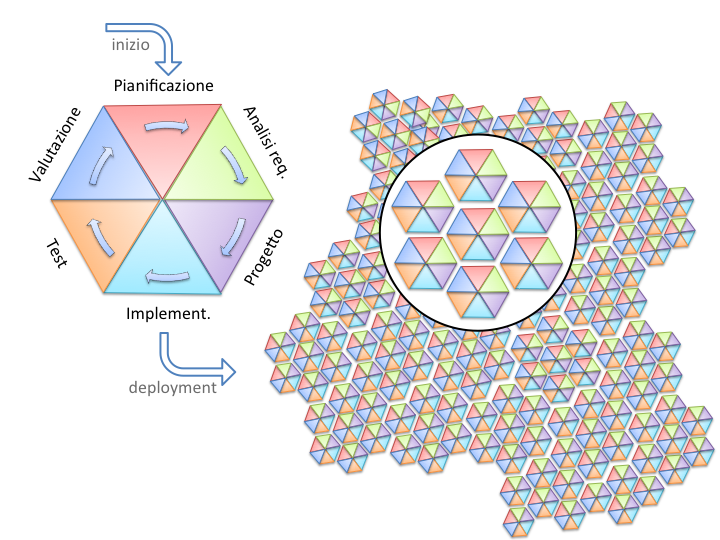
\includegraphics[scale=0.5]{img/modello_incrementale.png}
		\caption{Rappresentazione del modello incrementale\protect\footnotemark}
		\label{fig:modello_incrementale}
	\end{figure}

	\footnotetext{Fonte in \S\ref{rifinfo}}
	
    \include{sections/requisiti_sistema}
    \section{Configurazione}\label{configurazione}

Su richiesta di \II, tutti i servizi sono stati configurati sotto forma di container. È quindi possibile avviarli su macchine fisiche differenti, ma collegate in rete fra loro, con Docker.\\
Sempre sotto richiesta di \II viene utilizzato Rancher come software per la gestione dei container, quindi questa guida verterà principalmente sulla configurazione di \progetto utilizzando Rancher. %TODO riverere frase per ripetizione

\subsection{Requisiti di sistema}

	Non sono necessari particolari requisiti in modo da poter configurare e utilizzare il nostro prodotte, tuttavia valgono i requisiti minimi dei sistemi di terze parti che vengono utilizzati da \progetto.

	\subsubsection{Software}
		\begin{itemize}
			\item Docker\footnote{\url{https://docs.docker.com/v17.09/datacenter/ucp/2.1/guides/admin/install/system-requirements}}: è necessario avere installata e configurata correttamente almeno la versione v18.09.
			\item Docker Compose\footnote{\url{https://docs.docker.com/compose/install/}} :  nel caso si decidesse di utilizzare Docker Compose per l'avvio dei container è consigliata l'installazione e configurazione corretta della versione v3.7.
			\item Kubernetes\footnote{\url{https://kubernetes.io/docs/setup/independent/install-kubeadm}}: nel caso si decidesse di utilizzare Kubernetes per la gestione dei container è consigliata l'installazione e configurazione corretta della versione v1.13.
			\item Rancher\footnote{\url{https://rancher.com/docs/rancher/v2.x/en/installation/requirements/}}: nel caso si decidesse di utilizzare Rancher per la gestione grafica di oggetti Kubernetes contenenti i container Docker, è consigliata l'installazione e configurazione della versione v2.1.4.
			\item Kafka\footnote{\url{https://docs.confluent.io/current/installation/system-requirements.html}}: è necessario avere installata e configurata correttamente almeno la versione v2.12.
			\item GitLab\footnote{\url{https://git.ucd.ie/help/install/requirements.md}} 11.7
			\item Redmine\footnote{\url{https://www.easyredmine.com/faq/technical-info/176-hardware-and-software-requirements-for-server-solution}}: durante lo sviluppo di \progetto abbiamo utilizzato 4.0.1
		\end{itemize}
	
	%TODO rivedere
	GitLab e Redmine sono componenti esterne a \progetto, tuttavia vengono citate in quanto è possibile configurare tutto il progetto in un ambiente unico.\\
	Le versioni specificate possono essere trovate anche nella sezione ``Requisiti di vincolo'' del documento \AdRv.
	
	\subsubsection{Hardware}
	Per \progetto~non sono necessari ulteriori requisiti a livello hardware particolari se non quelli di cui hanno bisogno i software precedentemente elencati.

\subsection{Mappatura delle porte}
Per la configurazione di ciascun tipo servizio abbiamo deciso di dare un range di porte da poter esporre in modo tale da effettuare una separazione a logico.\\
Questa regola non influisce col corretto funzionamento di \progetto ma è solamente per non assegnare le porte in modalità casuale e facilitare le analisi di eventuali errori come anche la facile manutenzione e aggiunta di servizi.

La suddivisione delle porte è la seguente:

\begin{table}[H]
	\centering
	\begin{paddedtablex}[1.3]{\textwidth}{YYY}
		\thead{Servizio} & \thead{Porta inizio} & \thead{Porta fine}\\\toprule
		Software di terze parti& 30000& 30029\\\hline
		Kafka e servizi correlati& 30030& 30059\\\hline
		Producer& 30060& 30089\\\hline
		Consumer& 30090& 30119\\\hline
		Gestore personale& 30120& 30149\\
	\end{paddedtablex}
	\caption{Suddivisione delle porte}
\end{table}

La suddivisione che abbiamo utilizzato durante lo sviluppo ed alla consegna del progetto prevede la seguente esposizione delle porte:

\begin{table}[H]
	\centering
	\begin{paddedtablex}[1.3]{\textwidth}{YYY}
		\thead{Servizio} & \thead{Porta interna} & \thead{Porta esposta}\\\toprule
		Redmine& 3000& 30000\\\hline
		GitLab& 80& 30001\\\hline
		Kafka& 9092& 30030\\\hline
		Producer GitLab& 5000& 30060\\\hline
		Producer Redmine& 5000& 30061\\\hline
		Consumer Telegram& 30090& \\\hline
		Consumer Email& 30091& \\\hline
		Producer Gestore personale& 30120& 5000\\\hline
		Consumer Gestore personale& 30121& \\
	\end{paddedtablex}
	\caption{Configurazione delle porte in fase di sviluppo e consegna}
\end{table}

Le specifiche relative alla configurazione delle porte in Rancher possono essere trovate nella pagina dedicata\footnote{\url{https://rancher.com/docs/rancher/v2.x/en/installation/references/}} sulla sezione della documentazione presente nel loro sito.

\subsection{Configurazione servizi principali container}

	\subsection{Webhook}
	Per il corretto invio dei webhook (in formato JSON) da parte dei software che comunicano con i nostri Producer è necessaria una piccola configurazione:
	
	\paragraph{Redmine}
	
		\subparagraph{Configurazione del plugin}
	
		scaricarlo nella cartella... 
		verificare in sezione admin in configurazioni parte amministratore...
	
	L'implementazione per Redmine si appoggia sul plugin \texttt{redmine\_webhook}, raggiungibile al link
	\url{https://github.com/suer/redmine_webhook}.
	
	Questo plugin implementa il concetto di Hook offerto dalla API di Redmine, inviando a un determinato URL
	un \gloss{payload} costituito da un file JSON quando un evento si innesca, contenente le informazioni relative
	a tale evento.
	
	Per installarlo su un'istanza di Redmine, seguire le istruzione riportate nel README presente nella repository.
	
		\subparagraph{Configurazione destinazione}
		Per aggiungere una destinazione del webhook per un progetto, andare nella sezione relativa al webhook all'interno del menu del progetto...
		...aggiungere la destinazione e premere add..
		%todo inserire immagine
	
		\subparagraph{Eventi supportati}
		\begin{itemize}
			\item Comments
		\end{itemize}
	
		
	\paragraph{GitLab}
		\subparagraph{Configurazione webhook nella rete locale}
		È necessario abilitare l'invio dei webhook a dispositivi presenti nella stessa rete dalla parte amministrativa.
		Questo può essere effettuato accedendo con un account con privilegi amministratore all'indirizzo:
		\begin{center}
			\texttt{\url{/admin/application_settings/network}}
		\end{center}
		Per abilitare questa funzionalità cliccare sul riquadro rappresentato nell'immagine e che si trova all'indirizzo sopra indicato.
		\begin{figure}[H]
			\centering
			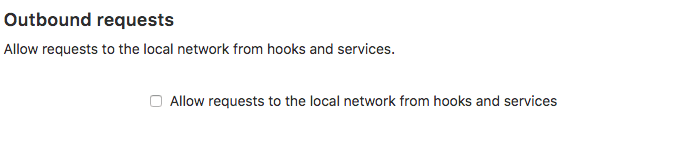
\includegraphics[width=13cm]{img/webhook_gitlab_setup.png}\\
			\caption[Webhook, GitLab]{Configurazione webhook con destinazione in rete locale}
		\end{figure}
		Ulteriori informazioni al riguardo possono essere trovate nella pagina\footnote{\url{https://docs.gitlab.com/ee/security/webhooks.html}} relativa a questo argomento sulla parte del sito relativa alla documentazione di GitLab.
		\subparagraph{Configurazione destinazione}
		Successivamente si può aggiungere indirizzo di destinazione un webhook al progetto andando sulle impostazioni:
		\begin{center}
			\texttt{Settings > Integrations}
		\end{center}
		Da qui si possono selezionare gli eventi di interessi per i quali i webhook verranno attivati (attenzione: \progetto~non supporta tutti gli eventi, solamente quelli richiesti da \II).
		Nel campo relativo all'URL di destinazione inserire l'indirizzo, con relativa porta (nel nostro caso quella specificata nella Tabella 2), su cui il Producer GitLab è in ascolto.
		\subparagraph{Eventi supportati}
		Per GitLab gli eventi supportati sono:
		\begin{itemize}
			\item Push events
			\item Comments
			\item Issues events
		\end{itemize}


---


	%TODO RIVEDERE
	La configurazione dei consumer e dei producer sono composte da file json contenti informazioni come ad esempio la mail di invio e la password relativa utilizzate per accedere al server mail.
	Queste possono essere modificate in modo tale da rispecchiare la configurazione che si vuole usare.
	
\subsection{Servizi aggiuntivi}
Aggiungere servizio necessario per il monitoraggio di kafka
Altri servizi per monitoraggio ?
    \section{Estendibilità}

\subsection{Aggiungere un Webhook}

Per aggiungere una nuova tipologia di Webhook, è sufficiente estendere l'interfaccia \texttt{Webhook}
e un eventuale \texttt{WebhookFactory} in caso si tratti di una nuova applicazione.

\begin{figure}[H]
    \centering
    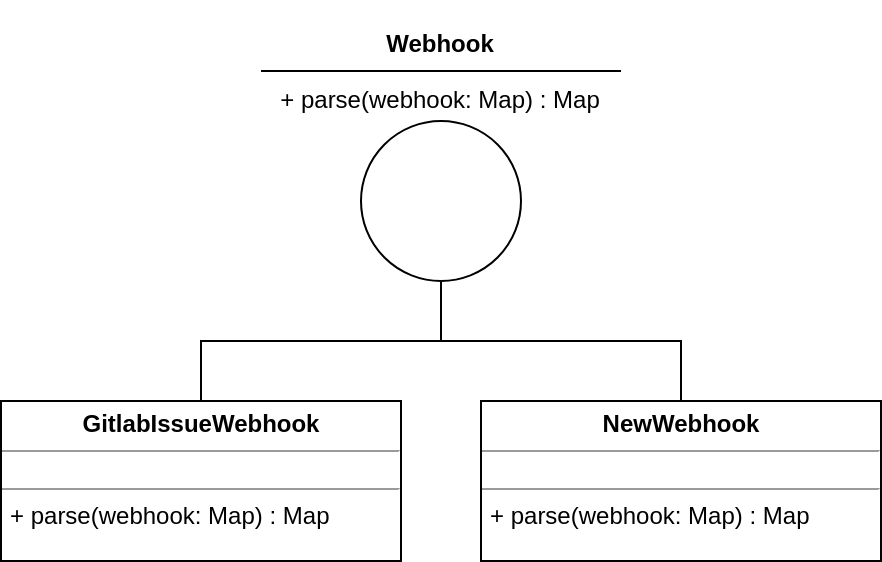
\includegraphics[width=0.7\textwidth]{img/EstensioneWebhook.png}\\
    \caption{Estendere un Webhook}
\end{figure}


\begin{figure}[H]
    \centering
    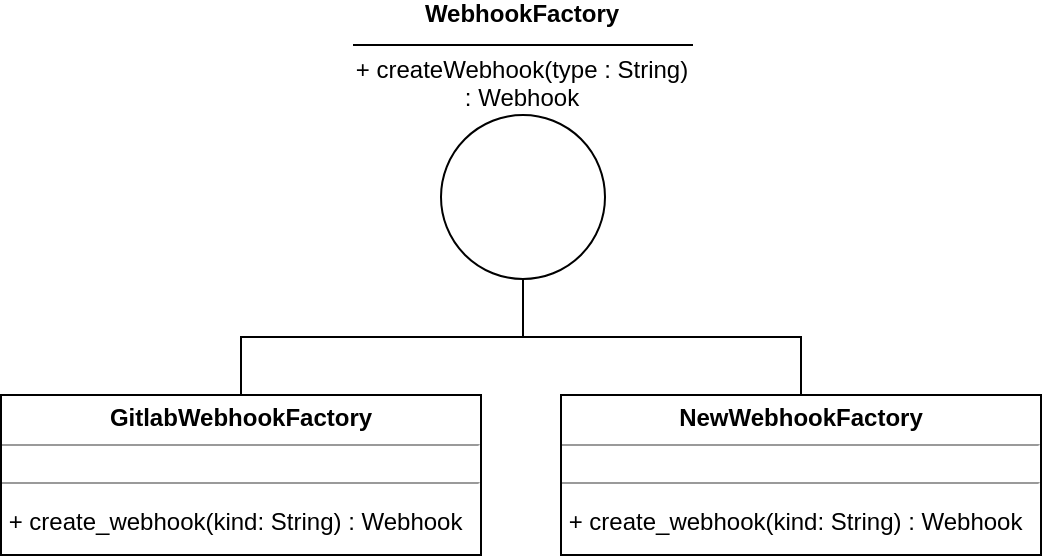
\includegraphics[width=0.7\textwidth]{img/EstensioneFactory.png}\\
    \caption{Estendere una Factory}
\end{figure}


    % \appendix
    % \newpage

\section{Consuntivo di periodo}	
	
	\subsection{Analisi dei Requisiti}
	Vengono riportate in seguito le ore di lavoro effettive relative al periodo di Analisi dei Requisiti.
	
	\begin{table}[H]
		\begin{detailtable}{\columnwidth}{m{3cm}YYYYYYY}
			\thead{Membro} & 
			\thead{Re} &
			\thead{Am} &
			\thead{An} &
			\thead{Pj} &
			\thead{Pr} &
			\thead{Ve} &
			\thead{Totale}\\\toprule\rowcolor{\tablegray}
			Ciprian Voinea & 11 (+3) & & 7 (-2) & & & 5 (-2) & 23 (-1)\\
			Laura Cameran & & 8 & 9 & & & 7 & 24\\\rowcolor{\tablegray}
			Matteo Marchiori & 7 (-1) & & 9 & & & 8 (+1) & 24\\
			Nicola Carlesso & 8 & & 10 (+1) & & & 7 & 25 (+1)\\\rowcolor{\tablegray} 
			Samuele Gardin & & 7 (-1) & 9 & & & 7 & 23 (-1)\\ 
			Timoty Graziero & & 7 (-1) & 8 (-1) & & & 9 (+2) & 24\\\bottomrule
		\end{detailtable}
		\caption{Tabella con le ore consuntivate nel periodo di Analisi dei Rischi}
	\end{table}
	
	Viene riportato in seguito il consuntivo relativo al periodo di Analisi dei Requisiti:
	
	\begin{table}[H]
		\begin{detailtable}{\columnwidth}{m{3cm}YY}
			\thead{Ruolo} & 
			\thead{Totale ore} &
			\thead{Costo in \euro}\\\toprule\rowcolor{\tablegray}
			Responsabile & 26 (+2) & 780,00 (+60,00)\\
			Amministratore & 22 (-2) & 440,00 (-40,00)\\\rowcolor{\tablegray}
			Analista & 52 (-2) & 1300,00 (-50,00)\\
			Progettista & & \\\rowcolor{\tablegray}
			Programmatore & &\\
			Verificatore & 43 (+1) & 645,00 (+15,00)\\\rowcolor{\tablegray}
			Totale & 143 (-1) & 3165,00 (-15,00)\\\bottomrule
		\end{detailtable}
		\caption{Tabella con il consuntivo del periodo di Analisi dei Rischi}
	\end{table}
	
	\subsection{Conclusioni}
	Non si ritiene opportuno aggiungere osservazioni in merito al discostamenti di orario rispetto a quanto preventivato.\\
	Questo primo consuntivo di periodo è di utilità per \gruppo\ di modo da poter osservare in modo oggettivo l'andamento del lavoro.\\
	Inoltre il preventivo iniziale viene presentato con questa prima versione del documento al proponente.
	
    % 
\newpage
\section{Attualizzazione dei rischi} \label{AttualizzazioneDeiRischi}
    Per dar senso ai rischi posti in analisi nel \PdP forniamo un resoconto di quanti si sono effettivamente verificati nei periodi di analisi dei requisiti e di progettazione della base tecnologica.\\
    Poiché i rischi cambiano dinamicamente durante lo svolgersi del progetto, questo appendice verrà aggiornato a intervalli regolari come stabilito nelle \NdP.
    I rischi che riportiamo sono quanto effettivamente abbiamo riscontrato nel portare a compimento le attività del progetto, possono anche differire da quelli presi precedentemente in analisi.\\

	\subsection{Classificazione}
    La classificazione dei rischi avverrà in modo simile a quella usata per l'analisi, riportando in questo caso anche la data in cui è stato riscontrato il rischio.
    Viene riportata per comodità del lettore la classificazione adottata per l'analisi dei rischi.

	A ciascun rischio viene assegnato un codice identificativo in modo da essere univoco e facilmente riconoscibile.

	Questo codice è:

	\begin{center}
		\texttt{[Tipologia][ID]-[Gravità][Probabilità][Classe]-[Data]}
	\end{center}

	composto da:
	
	\begin{itemize}
		\item \textbf{Tipologia}:
			\begin{itemize}
				\item \textbf{O}: organizzativo.
				\item \textbf{P}: personale.
				\item \textbf{R}: requisiti.
				\item \textbf{S}: strumentale.
				\item \textbf{T}: tecnologico.
			\end{itemize}

		\item \textbf{ID}: numero progressivo di tre cifre che inizia da uno (001 - 999).
		\item \textbf{Gravità}:
			\begin{itemize}
				\item \textbf{0}: accettabile.
				\item \textbf{1}: tollerabile.
				\item \textbf{2}: inaccettabile.
			\end{itemize}

		\item \textbf{Probabilità}:
			\begin{itemize}
				\item \textbf{0}: bassa.
				\item \textbf{1}: media.
				\item \textbf{2}: alta.
			\end{itemize}

		\item \textbf{Classe}: ci si riferisce ai livelli di rischio individuati dalla matrice in Figura \ref{fig:rischi}
			\begin{itemize}
				\item \textbf{0}: basso (verde).
				\item \textbf{1}: medio (arancione).
				\item \textbf{2}: alto (rosso).
			\end{itemize}
			
		\item \textbf{Data}: data in cui si è verificato il rischio, nel formato riportato nelle \NdP.
	\end{itemize}

	Ad esempio, con P001-021-2018-11-10 si può capire, seguendo la legenda, che si tratta del primo rischio del personale, di gravità accettabile, probabilità alta e un valore di classe medio, verificatosi in data 2018-11-10.

	\subsection{Lista rischi riscontrati}

	Per elencare i rischi viene utilizzata una struttura tabellare che indica nella prima riga il codice identificativo e il nome di ciascun rischio,
	mentre nelle righe successive vengono elencate e discusse la relativa descrizione, le strategie per la rilevazione e le eventuali contromisure e mitigazioni.\par

	La tabella potrà essere modificata in qualsiasi momento data la dinamicità dei rischi, e si sceglie di riportarli in ordine cronologico.


	\begin{table}[H]
		\begin{risktable}{\columnwidth}{m{4cm}m{11cm}}
			\thead{P002-122-2018-11-16} &
			Impreparazione del team a livello gestionale \\
			\rowcolor{\tablegray}
			\multicolumn{2}{X}{
				\textbf{Descrizione}: ci siamo ritrovati per iniziare a svolgere le attività del progetto, partendo dallo studio di fattibilità, senza la minima conoscenza dei ruoli.
			}\\
			\multicolumn{2}{X}{
				\textbf{Strategia adottata}: ognuno ha studiato i vari ruoli e le attività da svolgere per avere una visione globale di quanto sarebbe successo.
			}\\
		\end{risktable}
		\caption{Specifica rischio P002-122-2018-11-16}
	\end{table}

	\mydoublerule{\linewidth}{0pt}{2pt}

	\begin{table}[H]
		\begin{risktable}{\columnwidth}{m{4cm}m{11cm}}
			\thead{P003-122-2019-01-13} &
			Verifica e approvazione errata di documenti \\
			\rowcolor{\tablegray}
			\multicolumn{2}{X}{
				\textbf{Descrizione}: si sono verificate delle sviste durante la verifica dei documenti e l'approvazione è stata di conseguenza errata.
			}\\
			\multicolumn{2}{X}{
				\textbf{Strategia adottata}: abbiamo ricontrollato i documenti con più attenzione. Servirà dedicare più tempo alle attività di verifica.
			}\\
		\end{risktable}
		\caption{Specifica rischio P003-122-2019-01-13}
	\end{table}

	\mydoublerule{\linewidth}{0pt}{2pt}
	
	\begin{table}[H]
		\begin{risktable}{\columnwidth}{m{4cm}m{11cm}}
			\thead{S001-100-2019-01-18} &
			Problematiche hardware \\

			\rowcolor{\tablegray}
			\multicolumn{2}{X}{
				\textbf{Descrizione}: lo schermo del pc destinato alla presentazione è rimasto privo della retroilluminazione.
			}\\

			\multicolumn{2}{X}{
				\textbf{Strategia adottata}: abbiamo usato il pc di un altro membro del gruppo.
			}\\
		\end{risktable}
		\caption{Specifica rischio S001-100-2019-01-18}		
	\end{table}

	\mydoublerule{\linewidth}{0pt}{2pt}
	
	\begin{table}[H]
		\begin{risktable}{\columnwidth}{m{4cm}m{11cm}}
			\thead{O002-111-2019-02-09} &
			Mancanza di comunicazione con l'azienda \\

			\rowcolor{\tablegray}
			\multicolumn{2}{X}{
				\textbf{Descrizione}: la mancanza di una comunicazione abbastanza approfondita con la proponente ci ha portato a dover rivedere nel dettaglio i casi d'uso dell'\AdR.
			}\\

			\multicolumn{2}{X}{
				\textbf{Strategia adottata}: abbiamo previsto più momenti in cui comunicare con l'azienda, in modo da evitare ulteriori malintesi.
			}\\
		\end{risktable}
		\caption{Specifica rischio O002-111-2019-02-09}	
	\end{table}

	\mydoublerule{\linewidth}{0pt}{2pt}

	\begin{table}[H]

		\begin{risktable}{\columnwidth}{m{4cm}m{11cm}}
			\thead{P007-122-2019-02-12} &
			Pianificazione errata dei tempi \\
			\rowcolor{\tablegray}
			\multicolumn{2}{X}{
				\textbf{Descrizione}: ci siamo ritrovati con alcuni membri che avevano tutti gli esami previsti per il terzo anno da ultimare, altri con influenza e febbre. Questo ha portato a un ritardo non previsto nello svolgimento delle attività.
			}\\

			\multicolumn{2}{X}{
				\textbf{Strategia adottata}: abbiamo usato gli strumenti di pianificazione e coordinazione quali GitHub e Slack per coordinarci meglio e gestire il lavoro da ultimare.
			}\\
		\end{risktable}
		\caption{Specifica rischio P007-122-2019-02-12}
	\end{table}
    
	
	In seguito poniamo i rischi analizzati la cui priorità è cambiata nel corso del progetto:
	\begin{itemize}
	    \item \textbf{P005-011}: Intesa parziale tra i membri del team di sviluppo.
	    \item \textbf{R001-111}: Interpretazione errata dei requisiti: aggiunta o modifica di requisiti in corso di sviluppo.
	\end{itemize}

\end{document}
